\documentclass[10pt]{article}

% Pacotes extras necessários
\usepackage{amsmath}
\usepackage[lmargin=0.5in, rmargin=0.5in, tmargin=0.5in, bmargin=0.5in, includehead, includefoot]{geometry}
\usepackage{amsfonts}
\usepackage[utf8]{inputenc}
\usepackage[portuguese]{babel}
\usepackage{graphicx}
\usepackage{fancyhdr}
\usepackage{setspace}
\usepackage{listings}
\usepackage{url}
\usepackage{enumitem}
\usepackage{appendix}
\usepackage{subcaption}
\usepackage[dvipsnames]{xcolor}
\usepackage{tikz}
\usepackage{makecell}
\usetikzlibrary{positioning}

% Define estilo para listagens de código
\lstdefinestyle{mystyle}{
    language=Matlab,
    inputencoding=latin1,
    extendedchars=true,
    backgroundcolor=\color{white},
    basicstyle=\ttfamily\footnotesize,
    numbers=left,
    numberstyle=\tiny\color{gray},
    numbersep=5pt,
    tabsize=2,
    breaklines=true,
    keywordstyle=\color{blue},
    commentstyle=\color{green!60!black},
    stringstyle=\color{orange},
    frame=single,
    keepspaces=true,
    showspaces=false,
    showstringspaces=false,
    showtabs=false,
}
\lstset{style=mystyle}

\graphicspath{{./images/}}

\setlength{\parindent}{0pt}
\setstretch{1.5}

\DeclareMathOperator{\sen}{sen}
\DeclareMathOperator{\sinc}{sinc}
\newcommand{\Lap}[1]{\mathcal{L}\left\{#1\right\}}
\newcommand{\bm}[1]{\boldsymbol{#1}}

% Cabeçalho e rodapé em todas as páginas
\pagestyle{fancy}
\fancyhf{}
\fancyhead[L]{Relatório das simulações}
\fancyfoot[C]{\thepage}

% Dados do Grupo
\title{
    Trabalho Nº 06 - LS-MRAC \\
    \large COE603 - Controle Adaptativo
}
\author{
    Caio Cesar Leal Verissimo - 119046624 \\
    Leonardo Soares da Costa Tanaka - 121067652 \\
    Lincoln Rodrigues Proença - 121076407 \\
    Engenharia de Controle e Automação - UFRJ \\
    Rio de Janeiro, Rio de Janeiro, Brasil \\
    Julho de 2025
}
\date{}

\begin{document}

\maketitle

% Geração automática do sumário
\tableofcontents
\newpage

\section{Descrição do Algoritmo}

\subsection{Introdução ao Algoritmo}

Nesta seção, introduzimos o controlador adaptativo baseado no método dos mínimos quadrados (Least-Squares Model Reference Adaptive Control – LS-MRAC). Esse método é construído com base em uma função de Lyapunov que guia o projeto da lei de adaptação, visando garantir a estabilidade e a convergência do sistema.

\subsubsection{Função de Lyapunov}

Consideramos a seguinte função candidata de Lyapunov:
\[
2V(e, \tilde{\theta}) = \gamma e^T P e + \tilde{\theta}^T R^{-1}(t) \tilde{\theta}, \quad \text{com } R(0) = R^T(0) > 0
\]

Ao derivar essa função em relação ao tempo, obtemos:
\[
\dot{V} = -\gamma e^T Q e - \gamma |k_p| (\tilde{\theta}^T \xi)^2 + \gamma \tilde{\theta}^T \xi e_a + \tilde{\theta}^T R^{-1} \dot{\theta} + \frac{1}{2} \tilde{\theta}^T \dot{R}^{-1} \tilde{\theta}
\]

Lembrando que:
\[
\frac{d}{dt}[R R^{-1}] = \dot{R} R^{-1} + R \dot{R}^{-1} = 0 \quad \Rightarrow \quad \dot{R}^{-1} = -R^{-1} \dot{R} R^{-1}
\]

Substituindo na expressão de $\dot{V}$, temos:
\[
\dot{V} = -\gamma e^T Q e - \gamma |k_p| (\tilde{\theta}^T \xi)^2 + \tilde{\theta}^T \left( \gamma \xi e_a + R^{-1} \dot{\theta} - \frac{1}{2} R^{-1} \dot{R} R^{-1} \tilde{\theta} \right)
\]

\subsubsection{Leis de Adaptação Propostas}

Para garantir que a função de Lyapunov seja decrescente, propõe-se a seguinte lei de adaptação:
\begin{align*}
\dot{\theta} &= -\gamma R \xi e_a \\
\dot{R} &= -R \xi \xi^T R
\end{align*}

Com essa escolha, temos:
\[
R^{-1} \dot{R} R^{-1} = -\xi \xi^T
\]

E portanto:
\[
\dot{V} = -\gamma e^T Q e - \gamma |k_p| (\tilde{\theta}^T \xi)^2 + \frac{1}{2} (\tilde{\theta}^T \xi)^2
\]

\subsubsection{Condição para Decaimento de $V$}

Para garantir que $\dot{V} \leq 0$, é necessário que:
\[
\gamma > \frac{1}{2 |k_p|}
\]

Essa condição será retomada e aprofundada na próxima subseção, dedicada à análise formal de estabilidade.

\subsection{Análise de Estabilidade}

Nesta subseção, analisamos a estabilidade do controlador adaptativo por mínimos quadrados (LS-MRAC).

\subsubsection{Condição de Estabilidade}

A condição para garantir a estabilidade do sistema é dada por:
\[
\gamma > \frac{1}{2|k_p|}
\]

Sob essa condição, valem as seguintes propriedades:

\begin{itemize}
    \item $e \in \mathcal{L}_\infty$, \quad $\tilde{\theta}^T R^{-1} \tilde{\theta} \in \mathcal{L}_\infty$
    \item $e \in \mathcal{L}_2$, \quad $\tilde{\theta}^T \xi \in \mathcal{L}_2$
    \item $\omega, \xi, \dot{\xi} \in \mathcal{L}_\infty$
\end{itemize}

Consequentemente, a derivada da função de Lyapunov satisfaz:
\[
\dot{V}(e, \tilde{\theta}) \leq 0
\]

\subsubsection{Limitado de $R$ e $\theta$}

A limitação de $R$ e $\theta$ é obtida como segue:

Sabemos que $R(0) = R^T(0) > 0$. Assim, ao integrar a equação de atualização de $R^{-1}$, obtemos:
\[
\dot{R}^{-1}(t) = \xi \xi^T
\]
\[
R^{-1}(t) = R^{-1}(0) + J(t) > 0, \quad \forall t \geq 0
\]
onde:
\[
J(t) = \int_0^t \xi(\tau)\xi^T(\tau)\,d\tau
\]

Portanto, $R^{-1}(t) > R^{-1}(0)$, o que implica que $R(t) > 0$ para todo $t \geq 0$, ou seja, $R \in \mathcal{L}_\infty$. Assim, $\dot{\theta}$ e $\dot{R}$ também pertencem a $\mathcal{L}_\infty$.

\subsubsection{Análise pela Função de Lyapunov}

A partir da função de Lyapunov:
\[
2V = \gamma e^T P e + \tilde{\theta}^T R^{-1}(0) \tilde{\theta} + \tilde{\theta}^T J(t) \tilde{\theta}
\]

Cada termo acima pertence a $\mathcal{L}_\infty$, portanto:
\[
V \in \mathcal{L}_\infty \quad \Rightarrow \quad \tilde{\theta}^T R^{-1}(0) \tilde{\theta} \in \mathcal{L}_\infty \quad \Rightarrow \quad \tilde{\theta} \in \mathcal{L}_\infty
\]

\subsubsection{Convergência}

\begin{itemize}
    \item $\dot{e} \in \mathcal{L}_\infty \quad \Rightarrow \quad \lim_{t \to \infty} e(t) = 0$
    \item $\frac{d}{dt} (\tilde{\theta}^T \xi) \in \mathcal{L}_\infty \quad \Rightarrow \quad \lim_{t \to \infty} \tilde{\theta}^T \xi = 0$
\end{itemize}

\textbf{Portanto, todos os sinais permanecem limitados, o que garante estabilidade global uniforme.}

\subsection{Resumo do Algoritmo}

\begin{table}[htbp]
\centering
\begin{tabular}{|>{\bfseries}m{4cm}|m{6cm}|c|}
\hline
\textcolor{blue}{Subsistema} & \textcolor{blue}{Equação} & \textcolor{blue}{Ordem} \\
\hline
Planta & $y = P(s)\,u$ & $n$ \\
\hline
Modelo & $y_m = M(s)\,r$ & $n$ \\
\hline
Erro de rastreamento & $e_a = \text{sign}(k_p)(y - y_m)$ & \\
\hline
Filtros SV & 
$\begin{aligned}
\dot{\omega}_1 &= A_f \omega_1 + b_f u \\
\dot{\omega}_2 &= A_f \omega_2 + b_f y
\end{aligned}$ & $n-1$ \\
\hline
Regressor & $\omega^T = \begin{bmatrix} \omega_1^T & y & \omega_2^T & r \end{bmatrix}$ & \\
\hline
Filtro $\xi$ & $\xi = L^{-1}(s)[\omega]$ & $2n$ \\
\hline
Lei de controle & $u = \theta^T \omega + \dot{\theta}^T \xi$ & \\
\hline
Lei de adaptação & 
$\begin{aligned}
\dot{\theta} &= -\gamma R \xi e_a, \quad \gamma > \frac{1}{2|k_p|} \\
\dot{R} &= -R \xi \xi^T R, \quad R(0) = R^T(0) > 0
\end{aligned}$ & 
$\begin{aligned}
2n \\
\textcolor{red}{4n^2}
\end{aligned}$ \\
\hline
\end{tabular}
\caption{Resumo dos subsistemas, equações e ordens do sistema adaptativo}
\vspace{1em}
\textbf{Dimensão total do sistema:} \quad
\fcolorbox{magenta}{white}{$\displaystyle N = 8n + \textcolor{red}{4n^2} - 2$}
\end{table}

\newpage

\section{Resultados das Simulações}

Nesta seção, são apresentados os resultados das simulações realizadas com o sistema adaptativo proposto. A estrutura da simulação foi mantida, variando-se apenas um parâmetro por vez em relação à simulação base. Dessa forma, torna-se possível analisar a sensibilidade e influência de cada parâmetro no desempenho do sistema.

As simulações consideram as seguintes definições de planta e modelo de referência:

\begin{itemize}
    \item \textbf{Planta:} \( P(s) = \dfrac{k_p(s + 2)^2}{s^3} \), com \( k_p = \dfrac{1}{3} \)
    \item \textbf{Modelo de referência:} \( M(s) = \dfrac{1}{s + 1} \)
    \item \textbf{Filtro auxiliar:} \( \frac{1}{\Lambda(s)} = \dfrac{1}{(s + 0.5)(s + 1)(s + 1.5)} \)
\end{itemize}

A configuração de simulação base foi definida da seguinte forma:

\begin{itemize}
    \item Ordem do sistema: $n = 3$
    \item Tempo final da simulação: $t_{\text{final}} = 100$ s
    \item Passo de simulação: $st = 0.01$ s
    \item Condições iniciais: $y_0 = 0$, $\theta_0 = \mathbf{0}_{6\times1}$
    \item $\gamma = 20$, $R(0) = 20I$
    \item Sinal de referência: $r(t) =  3 + 10sqw(0.1 \pi t)$
\end{itemize}

A partir desta configuração base, foram realizadas as seguintes simulações adicionais:

\begin{itemize}
    \item Condições iniciais com $y_0 = 10$
    \item Condições iniciais com $\theta(0) = 0{,}9 \cdot \theta^*$
    \item $\gamma = 200$
    \item Matriz $R(0) = 200I$
    \item Sinal de referência com componentes senoidais: $r(t) =  3 + 10sqw(0.1 \pi t) + sin(t) + sin(3t) + sin(5t)$
\end{itemize}

Os resultados serão discutidos a seguir, com gráficos de comparação entre a saída do sistema e o modelo, além das estimativas dos parâmetros adaptativos e da evolução dos erros. Cada simulação destacará o impacto da variação considerada sobre o comportamento geral do sistema.

\newpage

\subsection{Simulação \#1 - Base}
\begin{figure}[h!]
    \centering
    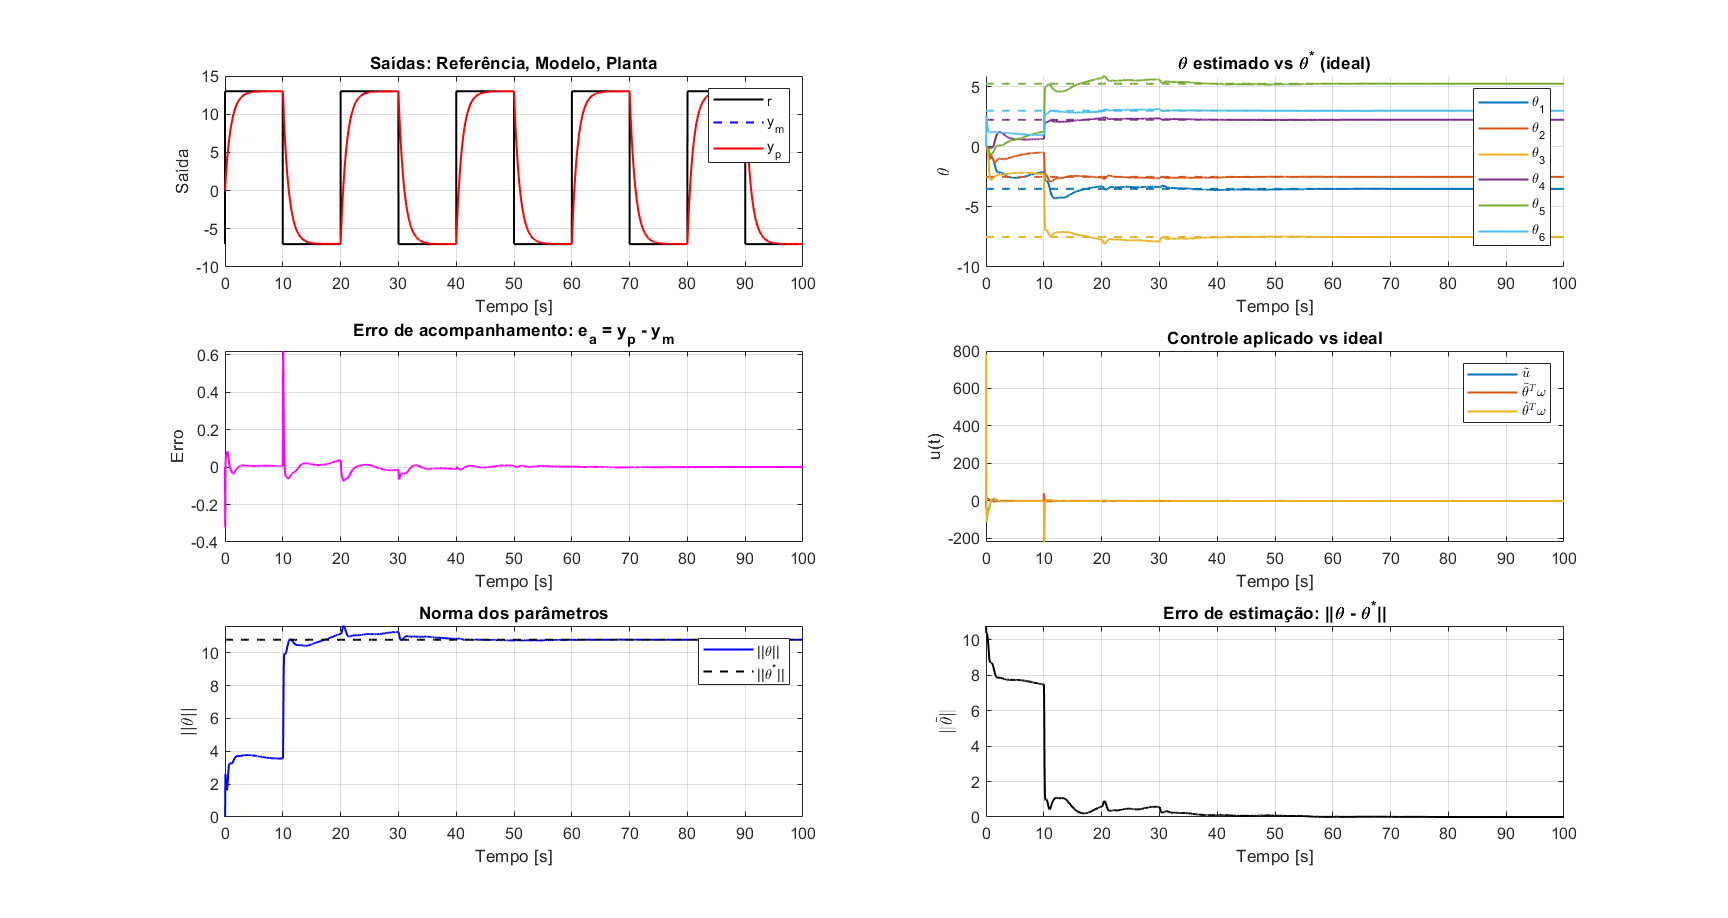
\includegraphics[width=0.85\textwidth]{img/sim01.png}
    \caption{Resultados da Simulação \#1}
    \label{fig:sim01}
\end{figure}

\subsection{Simulação \#2 - $y_0 = 10$}
\begin{figure}[h!]
    \centering
    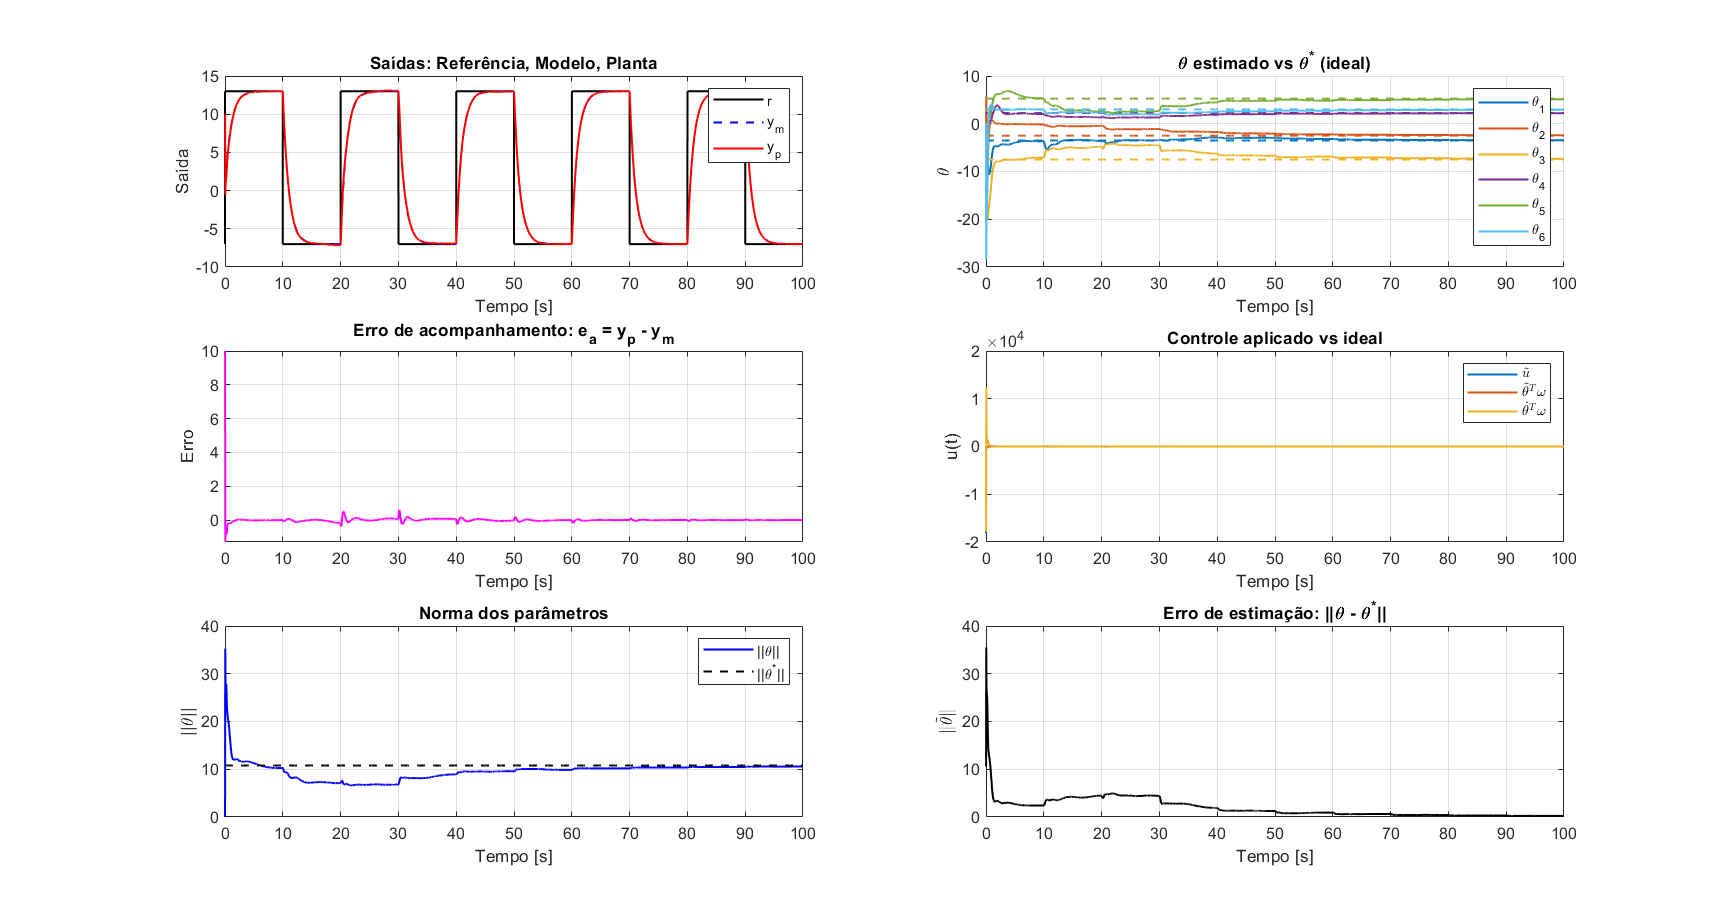
\includegraphics[width=0.85\textwidth]{img/sim02.png}
    \caption{Resultados da Simulação \#2}
    \label{fig:sim02}
\end{figure}

\newpage

\subsection{Simulação \#3 - $\theta(0) = 0.9\theta^{*}$}
\begin{figure}[h!]
    \centering
    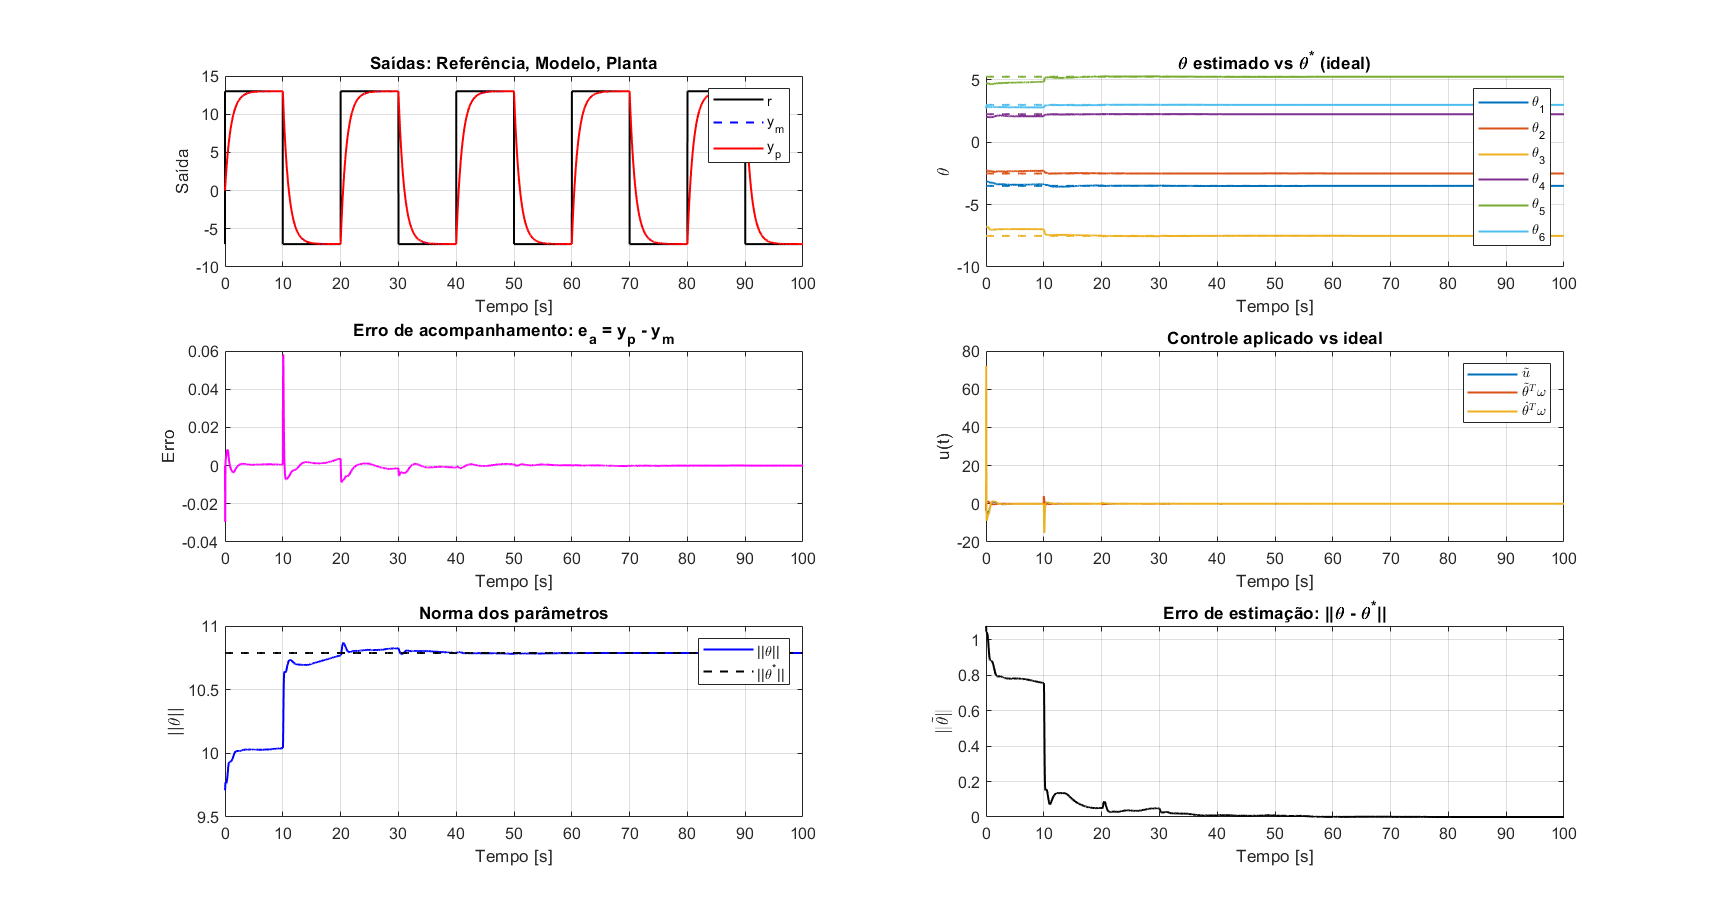
\includegraphics[width=0.85\textwidth]{img/sim03.png}
    \caption{Resultados da Simulação \#3}
    \label{fig:sim03}
\end{figure}

\subsection{Simulação \#4 - $\gamma = 200$}
\begin{figure}[h!]
    \centering
    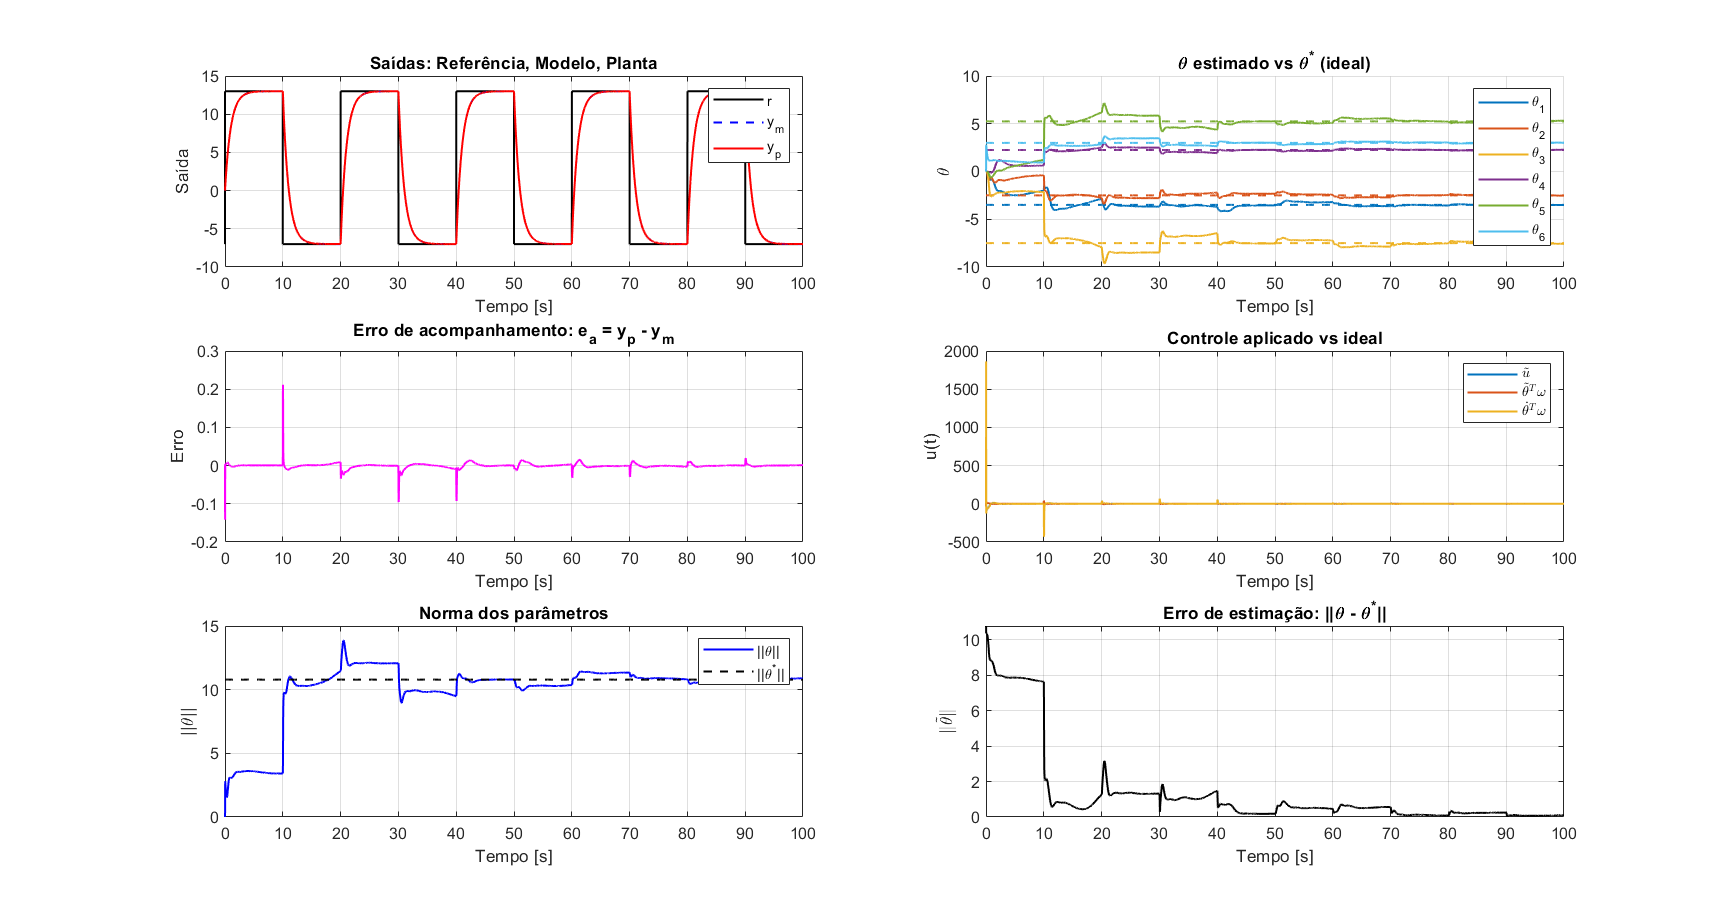
\includegraphics[width=0.85\textwidth]{img/sim04.png}
    \caption{Resultados da Simulação \#4}
    \label{fig:sim04}
\end{figure}

\newpage

\subsection{Simulação \#5 - $R(0)= 200I$ }
\begin{figure}[h!]
    \centering
    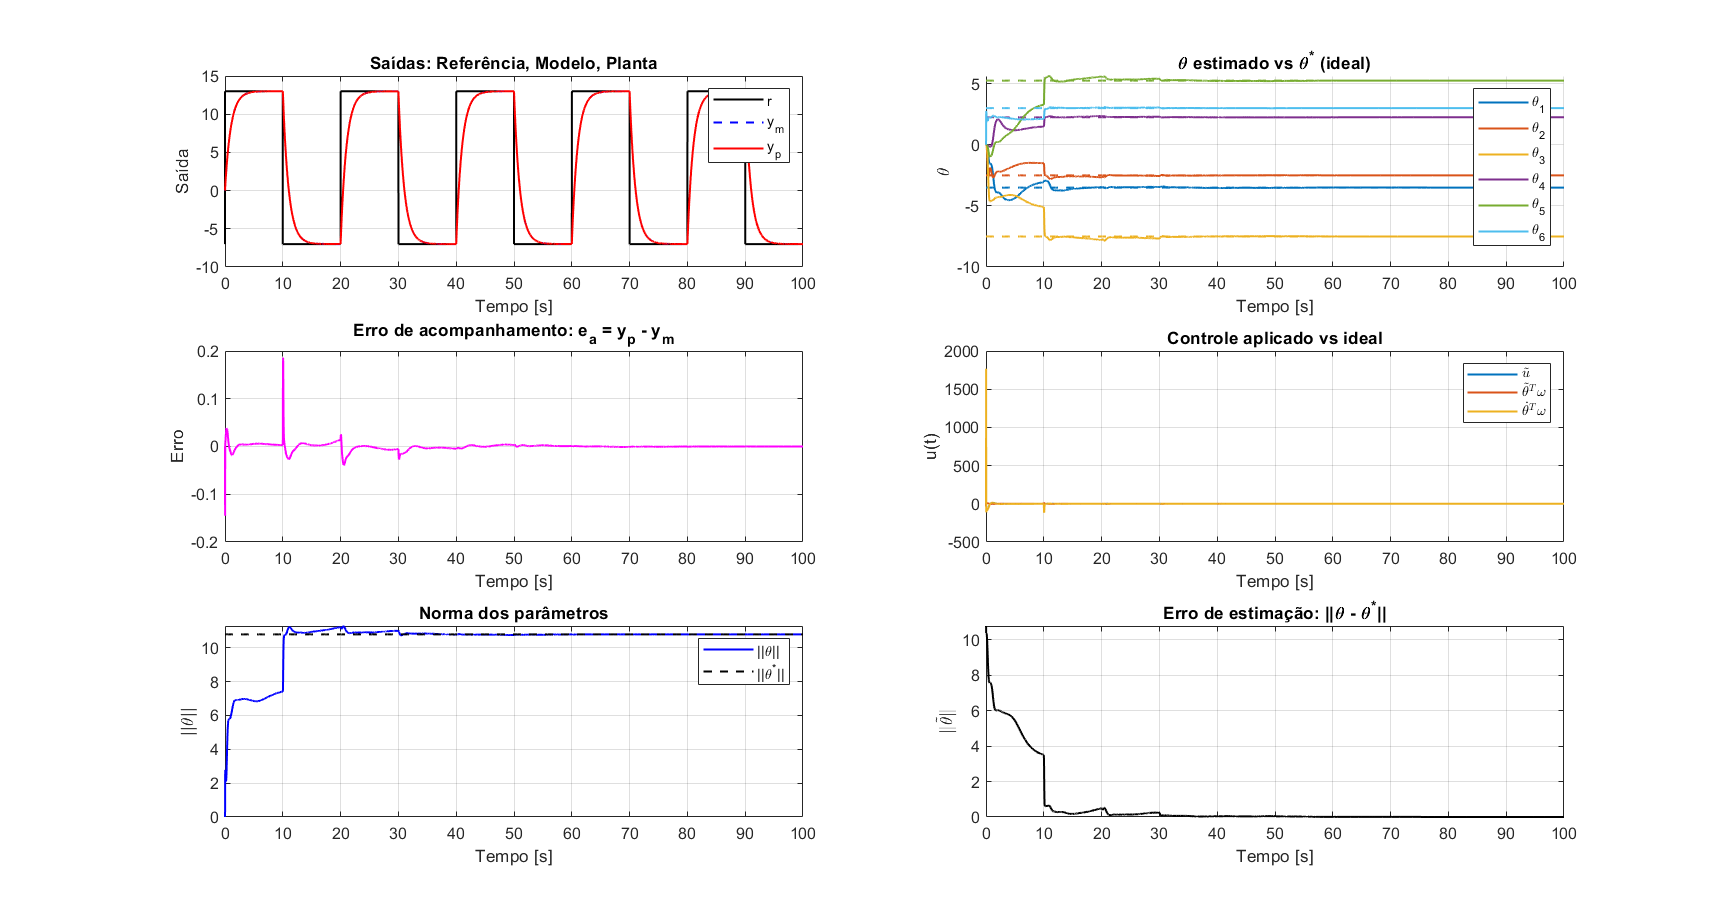
\includegraphics[width=0.85\textwidth]{img/sim05.png}
    \caption{Resultados da Simulação \#5}
    \label{fig:sim05}
\end{figure}

\subsection{Simulação \#6 - Mudança no Sinal de Referência}
\begin{figure}[h!]
    \centering
    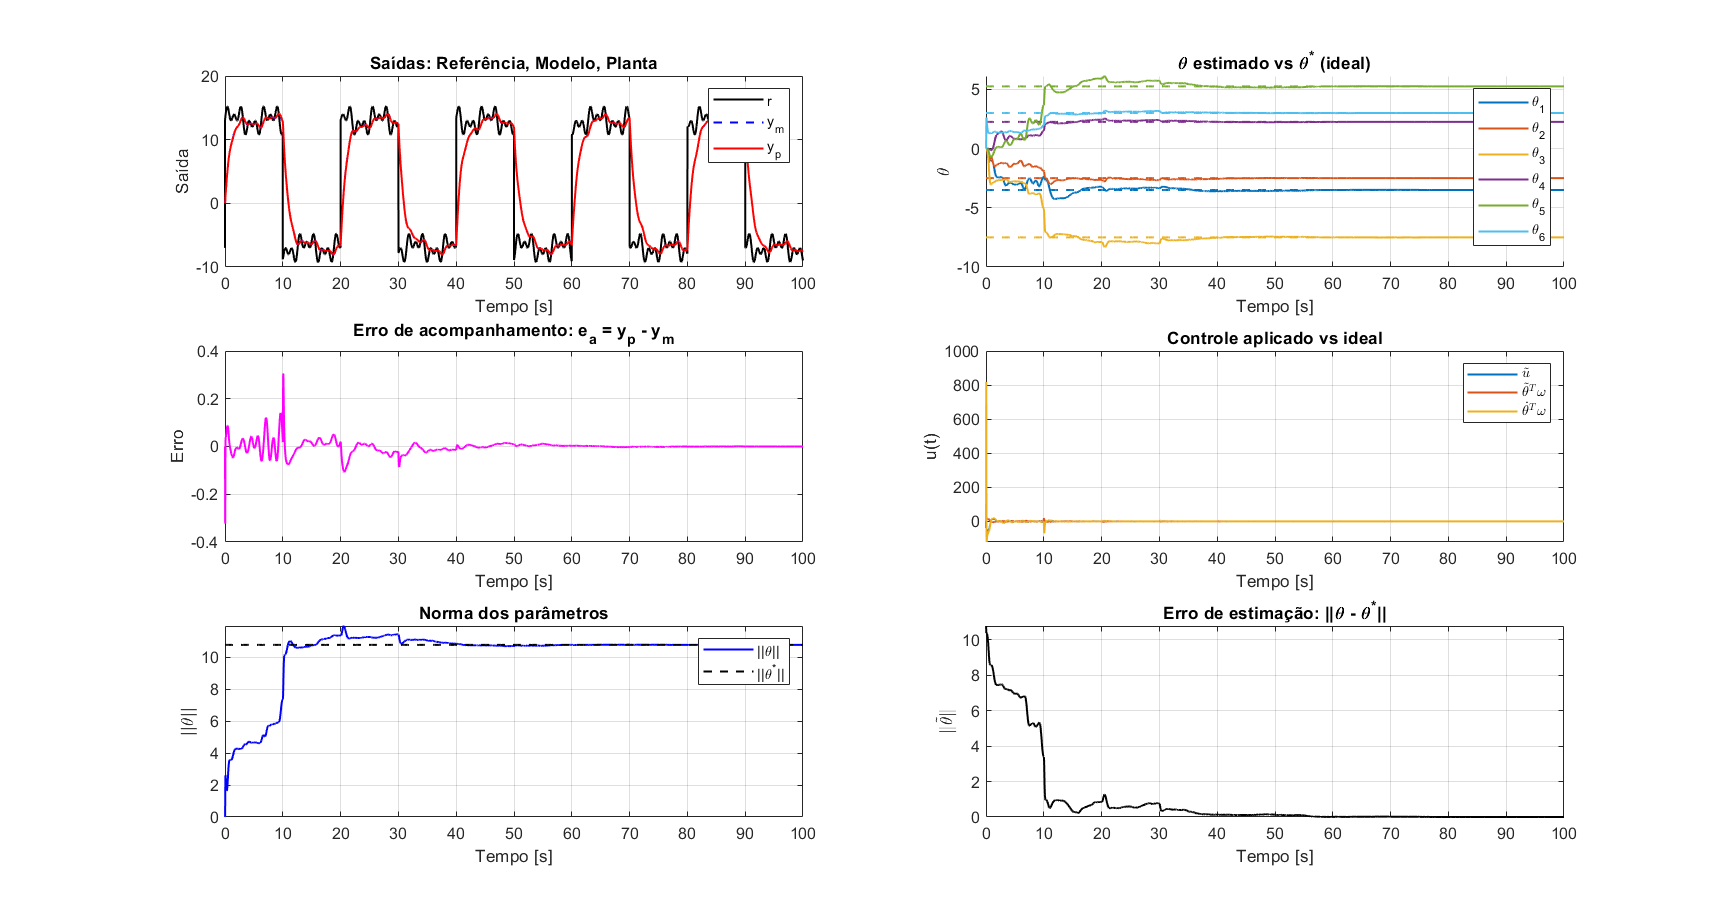
\includegraphics[width=0.85\textwidth]{img/sim06.png}
    \caption{Resultados da Simulação \#6}
    \label{fig:sim06}
\end{figure}

\newpage

\section{Discussão dos Resultados}

Nesta seção são analisados os comportamentos observados nas simulações do controlador LS-MRAC, com foco em robustez, velocidade de adaptação e sensibilidade a parâmetros.

\textbf{Simulação \#1 – Base:} O sistema acompanha a referência $y_m(t)$ com erro $e_a \rightarrow 0$ e convergência suave dos parâmetros $\theta(t)$, validando estabilidade global uniforme.

\textbf{Simulação \#2 – $y_0 = 10$:} Perturbação inicial gera transiente acentuado, mas o rastreamento é rapidamente recuperado, demonstrando robustez frente a condições iniciais desfavoráveis.

\textbf{Simulação \#3 – $\theta(0) = 0{,}9\theta^*$:} Parâmetros próximos do ideal aceleram a convergência, com redução do erro e transiente mais curto. Boa estimativa inicial melhora desempenho, embora não seja essencial.

\textbf{Simulação \#4 – $\gamma = 200$:} Aumento do ganho de adaptação acelera a convergência, mas eleva a sensibilidade a ruídos. Há um compromisso entre rapidez e robustez.

\textbf{Simulação \#5 – $R(0) = 200I$:} Valor inicial elevado para $R$ reduz a agressividade inicial do estimador, resultando em adaptação mais conservadora, mas ainda convergente.

\textbf{Simulação \#6 – Referência Senoidal:} A introdução de componentes senoidais melhora a persistência de excitação, promovendo convergência mais clara e erro pequeno, mesmo com maior complexidade no sinal.

\vspace{0.5em}
\textbf{Conclusão:} As simulações confirmam os fundamentos do LS-MRAC: estabilidade, rastreamento preciso e adaptação eficaz. O sistema é robusto a variações iniciais e seus parâmetros podem ser ajustados para melhorar desempenho sem comprometer a estabilidade.

\end{document}
